%% Lee
%% In dissertation, change 
%    section* to chapter 
%    subsection* to section
%    subsubsection* to subsection


%\chapter{Technical Approach}
\section{Technical Approach}
\label{chap-four}

The goals of this work is to research and design an ASIC based solution implemented using 3DIC technology able to support at or near real-time smultaneous 
processing of multiple ANNs. 
To achieve a \iffalse 20X \fi power/performance improvement over GPU's and potentially other solutions employing 3D DRAM, this work
needs to provide both a power and bandwidth improvement. 
This will be achieved by keeping the entire solution within the physical footprint of a 3DIC die stack \cite{tsai2008design}.
To achieve this goal, the solution will employ a custom organized 3D-DRAM to provide the required capacity along with custom management and processing
layers to perform all the computations associated with the multi-ANN application within the 3DIC die stack.
To provide the required bandwidth, this work will research a custom organized DRAM and data structures which will allow the processing layers
to perform all the ANN computations with direct access to the DRAM.
The combination of custom organized DRAM along with custom data structures will eliminate the requirement to store or cache the ANN data in 
local SRAM thus providing additional silicon to be applied to the computational units.
By keeping the solution within the 3DIC footprint, this work avoids the bandwidth loss due to input/output (IO) pin density reduction
associated with communicating off chip.
This work will employ high density TSV technology to provide the necessary communication bandwidth between main memory and the computational units.
These low capacitance TSV connections will reduce power dissipation compared to an off-chip IO solution whilst keeping the power dissipation within 
manageable limits.
By keeping within the 3DIC footprint, this work anticipates that even when including the usual system infrastructure this work will provide
a solution to applications that have significant size and power constraints.

Our proposed solution shown in \fref{fig:example 3DIC solution} includes a 3D-DRAM on top of a stack of custom die which includes a 
DRAM management layer and additional processing layers.
The die will be connected using through silicon vias (TSV).
The custom DRAM is sub-divided into smaller DRAM's accessed through individual ports. These ports include multiple banks and pages.
Each port is controlled by a port manager module.
The port manager reads operation units known as work units from a local instruction memory.
The work units identify the function, the memory locations to be streamed and the destination processing layer.
The port manager first transmits a configuration packet to the processing layer identifying the functions to be performed and
how the operands will be presented on the stack communication bus.
The port manager then streams the operands to the processing layer. The processing layer sends the result back to the management layer where the result
is directed to the appropriate DRAM port for storage.
The management layer may include:
\begin{itemize}
  \itemsep0em 
  \item a cluster CPU which is responsible for uploading the work unit instruction memory and to perform any operations more suited to a CPU
  \item port managers each controlling configuring the processing layer PE and streaming the operands and coalescing results back to DRAM
  \item a network-on-chip for communicating results to other port managers within the management layer 
\end{itemize}
\vspace{-1mm}
%%An example overall block diagram, die stack, communication bus (stack bus) and PE block diagram can
%%be seen in \fref{fig:example 3DIC solution}. %\fref{fig:blockDiagram}, \fref{fig:dieStack}, \fref{fig:stackBus} and \fref{fig:PeBlockDiagram} respectively.
%%This will be the starting point for our research.

The target neural networks will be analyzed for storage requirements and access patterns.
To achieve this, the target applications will be sub-divided into specific ANNs, such as BsB and cogent confabulation.
These ANNs will be further sub-divided into primitive operations, such as convolutions on an image region-of-interest or BsB processing of a character image etc..
These primitive operations will be analyzed to determine the optimum DRAM organization and data structures.
Of particular interest will be access patterns associated with cogent confabulation. The accessing of the cogent confabulation knowledge base matrices is 
not deterministic and it is this works intention to analyze access patterns and research options for sparce matrix storage and access.
It is anticipated that the access patterns will strongly influence the design of the sparse matrix storage method.

This combination of DRAM organization and data structures will be researched to ensure an acceptable level of bandwidth utilization
is obtained when accessing data in the DRAM.
The system will be further analyzed for power dissipation under the target applications.
This combination of specific DRAM organization and data structures makes this work unique.
The target applications will then be simulated to verify the system performance meets our anticipated results.

\begin{figure}
\centering
\captionsetup{justification=centering}
\vspace{0.5cm}
\begin{subfigure}{.7\textwidth}
  \centering
  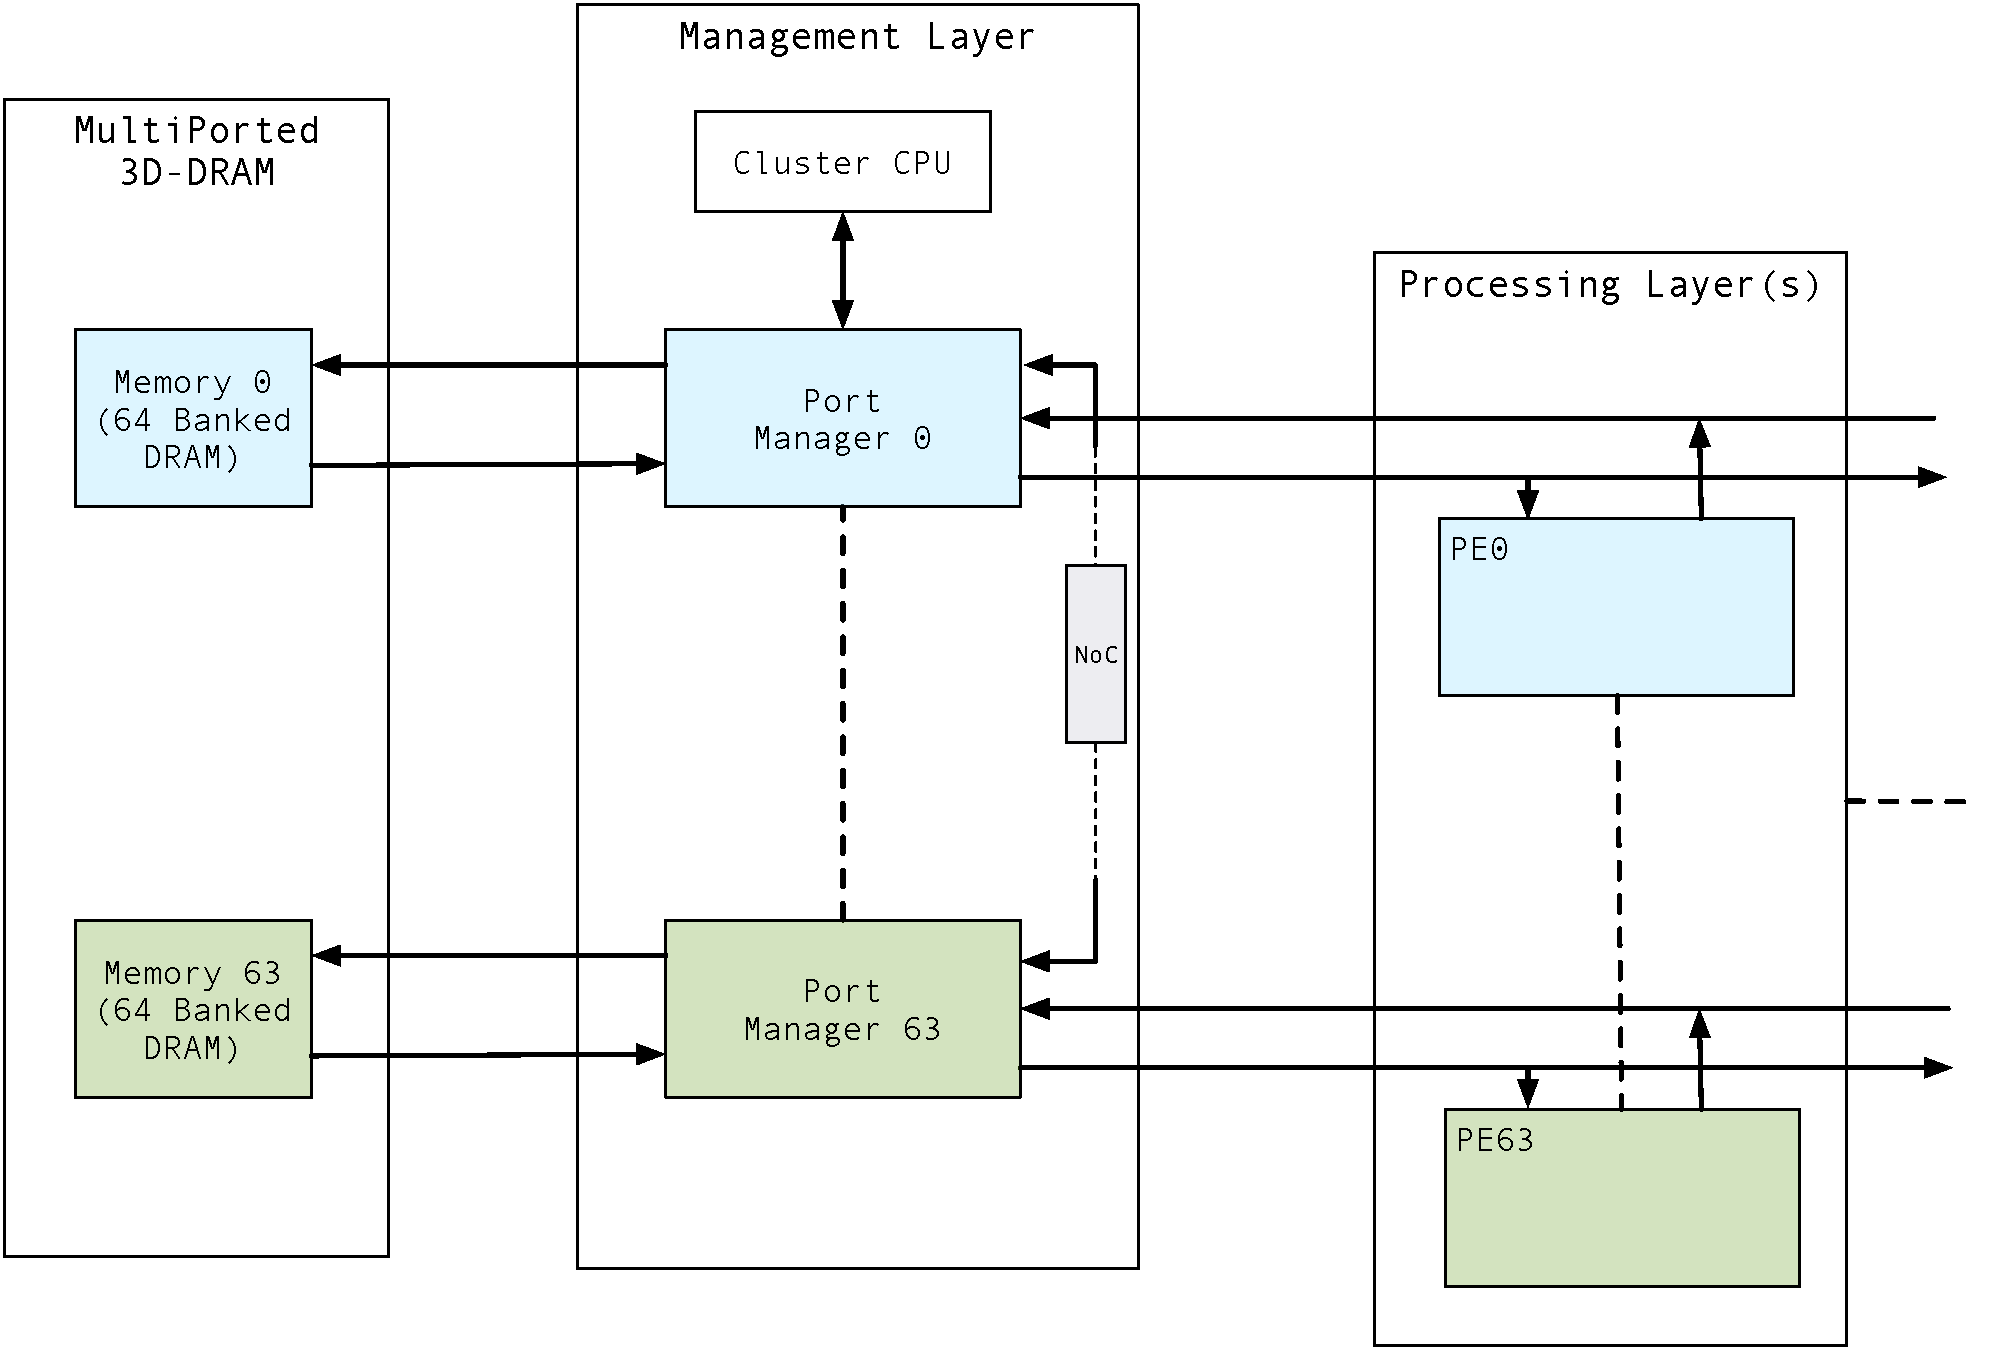
\includegraphics[width=0.60\textwidth]{Chapter-4/figs/BlockDiagram}
  \caption{System block diagram}
  \label{fig:blockDiagram}
\end{subfigure}%
\vspace{0.25cm}
\begin{subfigure}{.8\textwidth}
  \centering
  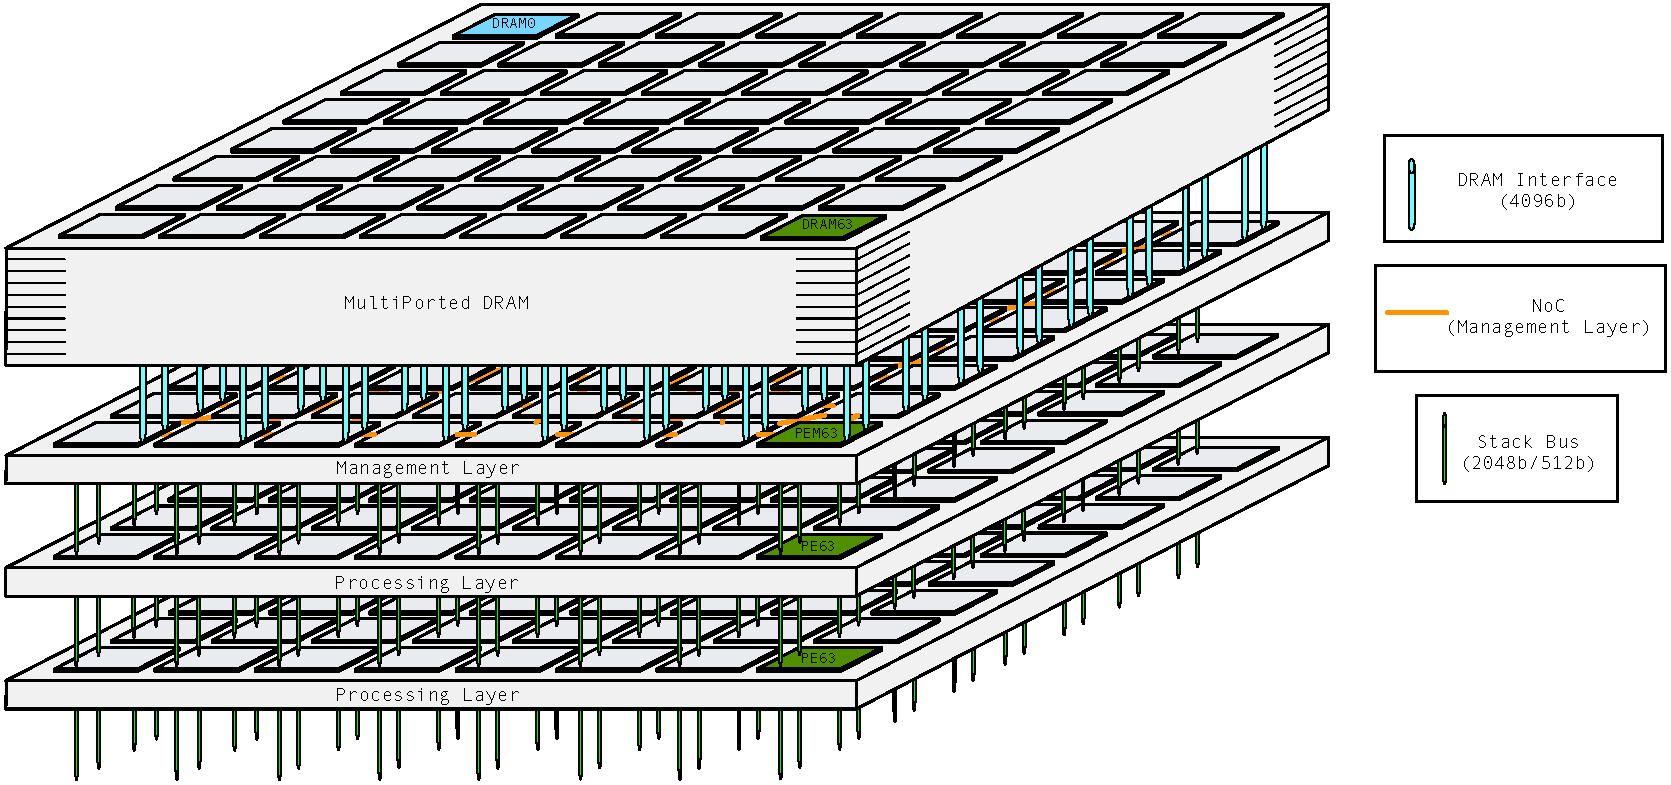
\includegraphics[width=0.55\textwidth]{Chapter-4/figs/DieStack}
  \caption{Die stack}
  \label{fig:dieStack}
\end{subfigure}
\vspace{0.25cm}
\begin{subfigure}{.9\textwidth}
  \centering
  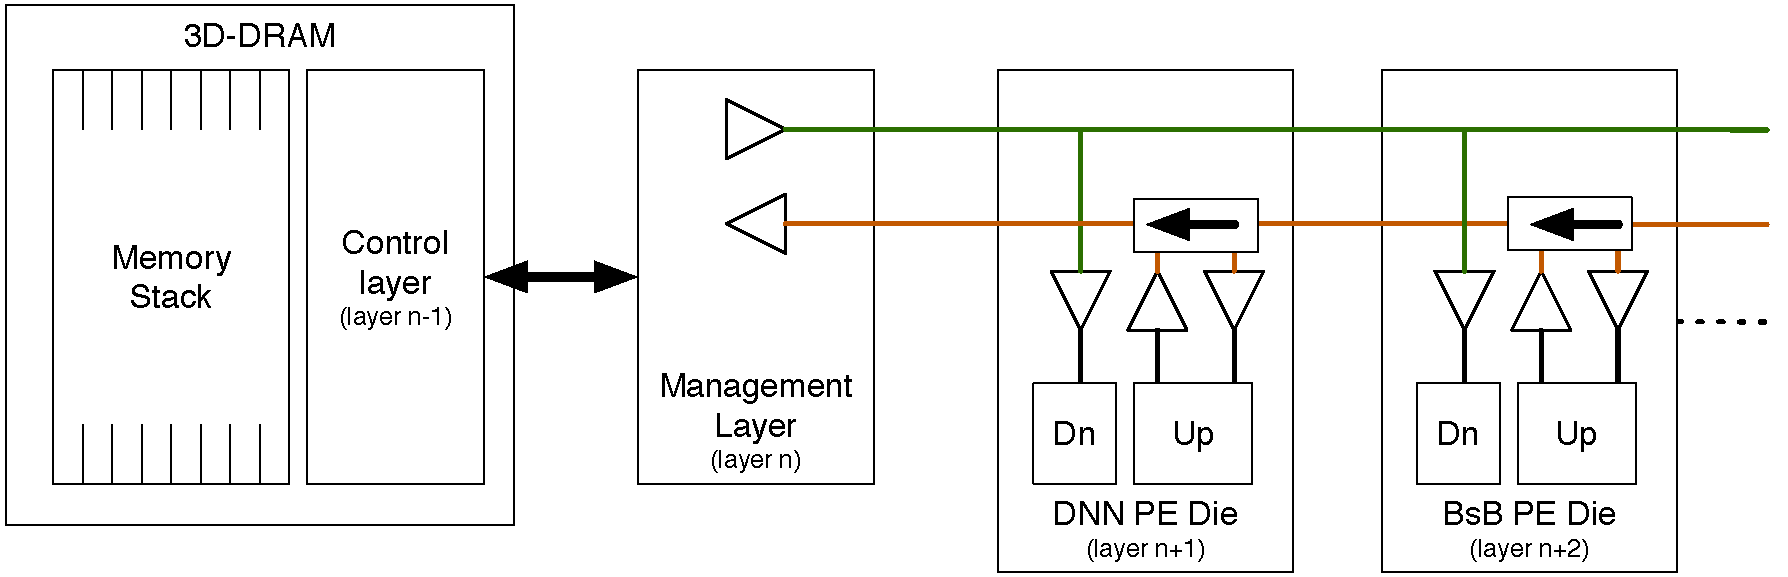
\includegraphics[width=0.85\textwidth]{Chapter-4/figs/StackBus}
  \caption{Stack Bus}
  \label{fig:stackBus}
\end{subfigure}
\begin{subfigure}{.7\textwidth}
  \centering
  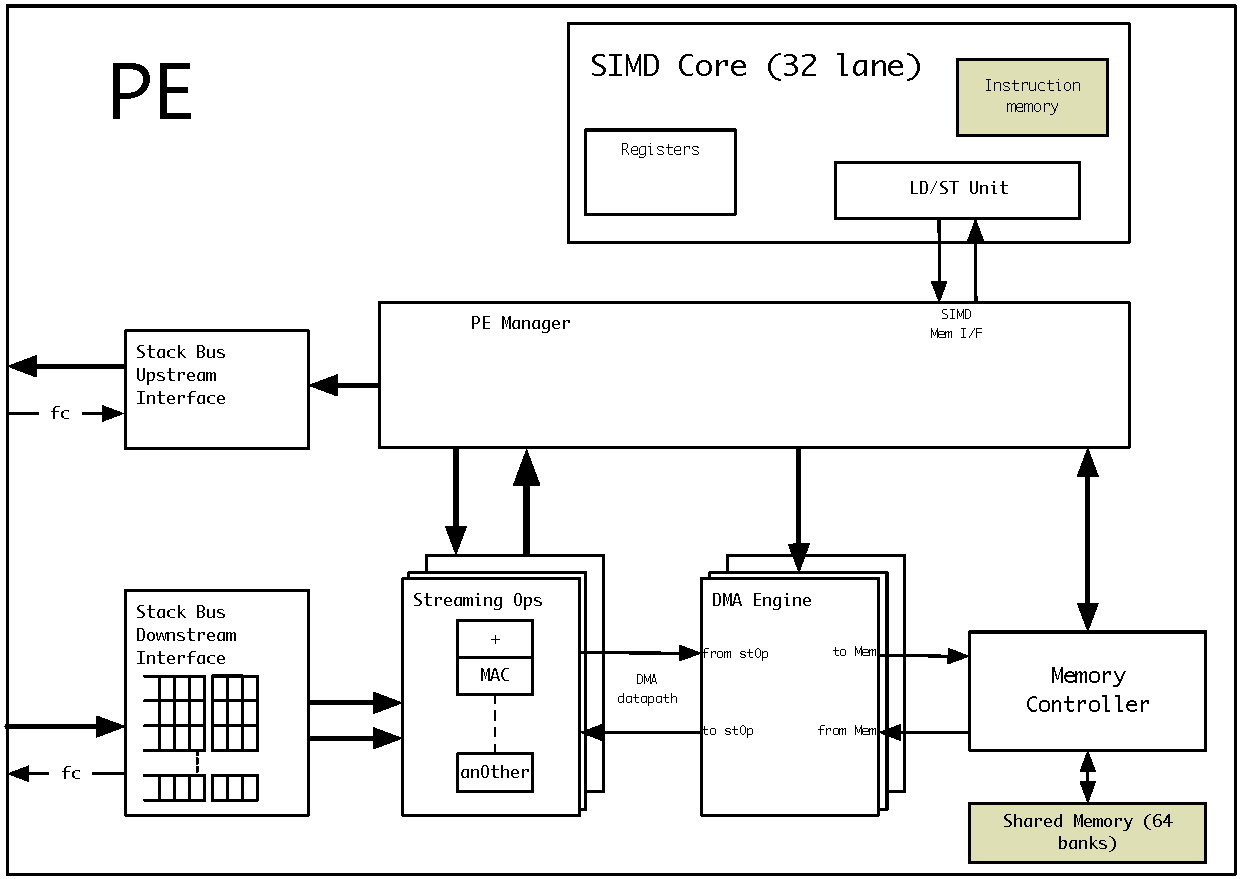
\includegraphics[width=0.6\textwidth]{Chapter-4/figs/PE}
  \captionsetup{justification=centering, skip=3pt}
  \caption{PE block diagram}
  \label{fig:PeBlockDiagram}
\end{subfigure}
\caption{Example 3DIC solution}
\label{fig:example 3DIC solution}
\end{figure}



